%TC: macro \marginfootnote [other]
%TC: envir SCfigure [] other
%TC: macrocount beginSCfigure [figure]
\documentclass[11pt,twoside]{report}
\usepackage{preamble}
\setcounter{chapter}{4}
\graphicspath{{../img/}}
\def\includebibliography{}

\externaldocument{background}
\externaldocument{supercooled-liquids}
\externaldocument{morphometric-framework}
\externaldocument{appendix-full-geometry}
\externaldocument{appendix-bayesian}

\begin{document}
\chapter{Local structure in the hard sphere liquid}
\epigraph{\textbf{hardball 1.1} \emph{informal} Uncompromising and ruthless methods or dealings.}{Oxford English Dictionary (2019).}
\label{chapter:morphometric-applications}

This chapter applies the theory developed in the previous chapter to the treatment of local structures in the hard sphere liquid.
Using the framework of many-body correlations and the morphometric approach, we calculate absolute free energies of local geometric motifs.
We find these to be in excellent quantitative agreement with molecular dynamics simulations across the liquid and supercooled liquid regimes.
We find a bimodality in the density library of states where fivefold symmetric structures appear lower in free energy than fourfold symmetric structures, and from a single reaction path predict an Arrhenius-like scaling of local relaxation dynamics.
The method provides a new route to assess changes in the free energy landscape at volume fractions dynamically inaccessible to conventional techniques.

The majority of this chapter consists of work published as Ref.\ \cite{RobinsonPRL2019}.
Towards the end of this chapter we introduce a new unpublished method for analytical calculations.
This has the potential to improve the efficiency of evaluating hard sphere free energies, as well as treat the saddles of the hard sphere energy landscape to make a connection with dynamics.
The details are somewhat technical however, so we have relegated them to Appendix \ref{appendix:bayesian}.

%% While `sphere' and `ball' are used interchangeably in physics (and colloquially), in geometry they refer to different things: balls $\ball^d$ are the solid objects whereas spheres are the boundaries $\partial \ball^d$.
%% As such, physicists really mean `hard balls' rather than hard spheres; the epigraph rang true for me as I undertook the work of this chapter.

\section{Introduction}

While mean-field theories provide insight into complex phenomena, physical accuracy is ensured only by a proper treatment of correlations.
For example, the simplest case of two-body correlations is at the foundation of predictive theories of the liquid state (section \ref{sec:liquid-state-theory}), colloids, and complex plasmas \cite{LikosPR2001,Ivlev2012}.
%, and some forms of active matter \cite{Bechinger2016}.
In particular, the thermodynamics of simple liquids with solely pairwise interactions can be exactly expressed in terms of two-body correlations (section \ref{sec:thermodynamic-routes}).
However, to resolve these integrated quantities \emph{spatially} into structural motifs, and \emph{temporally} into specific dynamical events, one needs to calculate many-body correlations.
While such a many-body approach may often be neglected in normal liquids, long-standing challenges such as the dramatic dynamical changes occurring in supercooled liquids approaching their glass transition \cite{BerthierRMP2011,RoyallPR2015} and phase transitions such as crystal nucleation \cite{RussoSR2012} call for a many-body description.

In the case of supercooled liquids, theories based on pair correlations such as the standard mode-coupling framework \cite{Gotze2009} fail to account for activated events thus predicting a spurious ergodicity breaking transition \cite{BrambillaPRL2009,HallettNC2018}.
Activated dynamics are often rationalised through collective (i.e.\ many-body) effects within contrasting thermodynamic and purely dynamic scenarios \cite{LubchenkoARPC2007,TarjusJPCM2005,BiroliPRL2006,JanssenPRL2015,SzamelPTEP2013,ChandlerARPC2010}.
These include exact mean-field results in high dimensions \cite{ParisiRMP2010,CharbonneauARCMP2017} whose relevance in finite-dimensional systems is hotly debated \cite{WyartPRL2017}.
A finite-dimensional theoretical description of many-body effects is therefore much needed.
We discussed the various theories mentioned above in more detail in chapter \ref{chapter:glass}.

However, many-body correlations are challenging to compute and typically combine both energetic and entropic contributions.
Physical insight can be gleaned by exploring the potential energy landscape of isolated clusters \cite{Wales2004,ArkusPRL2009}, but such methods are only exhaustive for small system sizes.
This limitation has been partly addressed by embedding clusters in a mean-field approximation of the surrounding liquid \cite{MossaJCP2003,MossaJNS2006}.
Nonetheless, this approach neglects by construction the intra-cluster entropic contributions that may dominate in the supercooled regime of interest.
Furthermore, computer simulations, which naturally deliver full many-body correlations are limited in the range of dynamics they can access, hampering an approach to the glass transition, except for recent developments with certain models \cite{BerthierPRL2016}.

In this chapter we place theoretical predictions of many-body local structure on a fundamentally more rigorous footing using inhomogeneous liquid state theory \cite{EvansAP1979}, which we reviewed in section \ref{sec:dft} and advanced in chapter \ref{chapter:morphometric-framework}.
Using the morphometric approach to treat the many-body interactions between a local subsystem and the remaining liquid, we can directly access the many-body \textit{free} energy of local arrangements of particles.
This allows us to predict the populations of specific local structures%
\marginfootnote{We have actually already seen two simple examples of this in section \ref{sec:framework-numerics}: the concentrations of the dimer ($n=2$) and triangle ($n=3$) structures in \eqref{eq:coordination} and \eqref{eq:triangle-concentration}.
The aim of this chapter is to generalise to arbitrary $n$.}
in the bulk system across the entire liquid phase, and beyond the dynamically accessible supercooled regime.

\section{Free energy of local structures}

%\subsection{Concentrations of local structure}

%% How do we define a local structure?
%% Most of the literature on structure in amorphous systems falls into one of either two categories
%% Almost all methods for Common methods:
%% \begin{itemize}
%%   \item Bond orientational order parameters
%%   \item Bond networks: take some bond detection algorithm (voronoi,
%% Fom the partition function of the potential of mean force
%% Suppose we have a definition of a
%% \end{itemize}

From the definition of the $n$-particle density \eqref{eq:n-particle-density-pdf} as a probability density function, the total number of a local structure in a system volume $V$ is
\begin{equation}\label{eq:structure-population}
  \mathcal{N}
  =
  \frac{1}{n!}
  \int_{\mathcal{Q}}
  \rho^n g^{(n)}(\vec{r}^n)
  \, d\vec{r}^n,
\end{equation}
where $\mathcal{Q}$ is the domain \emph{defining} the particular local structure.
In terms of the potential of mean force \eqref{eq:potential-mean-force} this would be written equivalently as
\begin{equation*}
  \mathcal{N}
  =
  \frac{1}{n!}
  \int_{\mathcal{Q}}
  \rho^n \exp{\left(-\beta\phi^{(n)}(\vec{r}^n)\right)}
  %e^{-\beta \phi^{(n)}(\vec{r}^n)}
  \, d\vec{r}^n,
\end{equation*}
which has a similar structure as the canonical partition function \eqref{eq:canonical-partition} so we can think of structure population $\mathcal{N}$ as being the equivalent partition function in our ensemble%
\marginfootnote{Formally, this is the \emph{semi-grand canonical ensemble} because there is a chemical potential $\mu$ for the bulk component, but also a fixed number of particles for the local component $n$.}.
From the latter observation we could define a free energy for the local structure from $-k_B T \, \ln{\mathcal{N}}$,
%% \begin{equation*}
%%   \beta F = - \ln{\mathcal{N}},
%% \end{equation*}
but we will find it more useful to define the free energy as an excess quantity.
Specifically, we exploit translational invariance of $\phi^{(n)}$ in the uniform liquid to integrate the centre of mass over the system volume, as in
\begin{equation}
  \mathcal{N}
  =
  \frac{\rho^n V}{n!}
  \int_\mathcal{D}
  g^{(n)}(\vec{r}^{n-1})
  \, d\vec{r}^{n-1},
\end{equation}
defining the internal structure space $\mathcal{D}$ through $\mathcal{Q} = \mathcal{D} \times V^d$.
The prefactor $\rho^n V$ is the trivial scaling of the ideal gas, so we define the free energy of the structure through the excess quantity%
\marginfootnote{Note: in previous chapters we used the symbol $F$ to refer to the Helmholtz free energy; here it will \emph{only} refer to the free energy of a local structure.}
\begin{equation*}
  e^{-\beta F}
  =
  \frac{\mathcal{N}}{\sigma^{d(n-1)} \rho^n V},
\end{equation*}
with powers of particle diameter $\sigma$ introduced to make the right-hand side dimensionless.
Note that $\mathcal{N} / V$ is the \emph{concentration} of the structure, so the right-hand side could be thought of as an excess concentration.
Written explicitly, the free energy of the local structure is
\begin{equation}\label{eq:local-structure-free-energy}
  \begin{split}
    \beta F
    &=
    -\ln{
      \left(
        \frac{1}{\sigma^{d(n-1)} n!}
        \int_{\mathcal{D}}
        g^{(n)}(\vec{r}^{n-1}) \, d\vec{r}^{n-1}
      \right)
    },
    \\
    &=
    -\ln{
      \left(
        \frac{1}{\sigma^{d(n-1)} n!}
        \int_{\mathcal{D}}
        \exp{\left(-\beta\phi^{(n)}(\vec{r}^{n-1})\right)}
        \, d\vec{r}^{n-1}
      \right)
    }.
  \end{split}
\end{equation}
Evaluating this free energy thus requires a closure for $\phi^{(n)}$, a definition of the structure to set integration limits through $\mathcal{D}$, and a method of actually doing the integration.

We calculate $\phi^{(n)}$ from its definition \eqref{eq:potential-mean-force} and using the morphometric \emph{ansatz} \eqref{eq:morph-ansatz} as a closure for $\Delta \Omega$.
Our focus is on $d=3$, so we use the virial route coefficients \eqref{eq:virial-coefficients} with the Carnahan-Starling equation of state \eqref{eq:cs-pressure} because the resulting correlation functions are highly accurate (cf.\ section \ref{sec:framework-numerics}).
We have already seen how this equation of state is accurate at high densities (Fig.\ \ref{fig:swap-eos}), though it is worth emphasising that it must fail at some point setting limits on our approach.
%The pair correlation produced by these coefficients is self-consistent with CS at contact by construction; moreover, the new coefficients provide a theory that outperforms the older WBII approach across the whole range of distances typical of neighbouring particles (SM).
%This enables us to accurately model complex many-particle local structures.
We calculate the morphological quantities $\{V, A, C, X\}$ using an algorithm described in Ref.\ \cite{KleninJCC2011}, which we have extended to calculate curvature measures (see details in Appendix \ref{appendix:computational-geometry}).

In conventional energy landscape approaches, a structure%
\marginfootnote{Energy landscape approaches are actually more general than just pertaining to local structures, as they could in principle refer to the landscape of a macroscopic system as they do in e.g.\ mean field approaches (cf.\ section \ref{sec:mean-field-glass}).
  It is only in this context of small system sizes that they refer to local structures.}
would be defined by the region, or \emph{basin}, surrounding an energy minimum called the \emph{inherent state} \cite{StillingerPRA1982,StillingerS1995,Wales2004}.
Defining the location of the inherent state as
\begin{equation*}
  \vec{y}^*
  :=
  \argmin_{\vec{y} \in \mathcal{D}}{\left( \phi^{(n)}(\vec{y}) \right)},
\end{equation*}
with $\vec{y}$ as shorthand for $\vec{r}^{n-1}$.
The partition function would then be evaluated via a perturbation theory around the inherent state, i.e.\ from the Taylor expansion \cite{Wales2004}
\begin{equation*}
  \phi^{(n)}(\vec{y})
  =
  \phi^{(n)}(\vec{y}^*)
  + \frac{1}{2} (\vec{y} - \vec{y}^*) \cdot
  \nabla\nabla \phi^{(n)}(\vec{y}^*)
  \cdot (\vec{y} - \vec{y}^*)
  + \mathcal{O}(\vec{y}^3)
\end{equation*}
which is valid in the case of \emph{smooth} potentials where $\nabla \phi^{(n)}(\vec{y}^*) = 0$.
Then, \cite{Wales2004}
\begin{equation}\label{eq:harmonic-approximation}
  \begin{split}
    \int_\mathcal{D} e^{-\beta\phi^{(n)}(\vec{y})} d\vec{y}
    &\simeq
    e^{-\beta\phi^{(n)}(\vec{y}^*)}
    \int_\mathcal{D}
    \exp{\left( - \frac{\Delta\vec{y} \cdot \vec{H} \cdot \Delta\vec{y}}{2} \right)}
    \, d\vec{y}
    \\ &\approx
    \sqrt{ \frac{(2\pi)^{d(n-1)}}{\det \vec{H}} }
    e^{-\beta\phi^{(n)}(\vec{y}^*)}
  \end{split}
\end{equation}
where $\vec{H} = \nabla\nabla \beta \phi^{(n)}(\vec{y}^*)$ is the (positive-definite) Hessian matrix and $\Delta \vec{y} = \vec{y} - \vec{y}^*$, and in the latter line the integral is taken over all of space (as an approximation) using the multivariate Gaussian integral%
\marginfootnote{As a simplification in this step we ignored rigid rotations, which cannot be treated perturbatively in general.
We give the correct treatment of rotations in section \ref{sec:structure-definition}.}.
This method is variously referred to as the \emph{saddlepoint approximation}, \emph{Laplace's method} or the \emph{harmonic approximation} in different communities.
This approach fails in hard particle systems because the pair potential is pathological: $\nabla \phi^{(n)}(\vec{y}^*) \ne 0$, the Hessian generally has negative eigenvalues and the integral cannot be approximated over all of space.

As the hard sphere pair potential is singular, we require non-perturbative methods to evaluate the free energy which we will introduce in sections \ref{sec:local-library} and \ref{sec:reaction-paths}.
We will begin by proposing an operational definition for the structures so that we have a domain of integration.

\section{How do we define a local structure?}
\label{sec:structure-definition}

An ideal definition of local structures would exactly partition the phase space of possible states within the liquid, so that the free energy and configurational entropy with varying lengthscale (through $n$) could be assessed.
This would allow direct comparison with the mean-field of glass (sections \ref{sec:mean-field-glass} and \ref{sec:finite-d-glass}), particularly with equations \eqref{eq:rfot-barrier} and \eqref{eq:rfot-xi}.
In an attempt to work towards this ideal, we develop an approximate coarse-graining scheme borrowing intuition from traditional energy landscape approaches.

Towards the end of the previous section we indicated an approach which treats structures as perturbations from inherent states.
This approach has been highly successful in advancing the understanding of colloidal and molecular clusters \cite{WalesJCP1994,DoyePRB2001}, liquids \cite{DoyeJCP1995,DoyeJPB1996,StillingerPRA1982}, glasses \cite{WalesN1998,StillingerS1995} and proteins \cite{Wales2004}.
To remain as close as possible to the spirit of this approach, we choose to define structures starting from energy minima.
The minima of $\phi^{(n)}$ occur around contact in hard spheres.
To justify this, consider that the dominant term in the morphometric approach \eqref{eq:morph-ansatz} is the volume term $pV$, which is minimised when particles are as compact as possible i.e.\ at contact; we cannot prove this rigorously, but we have yet to find a counter example.

\begin{SCfigure}
  \includegraphics[width=\linewidth,outer]{packings}
  \caption[Rigid spherical packings of up to 7 particles]{
    Rigid sphere packings for $3 \le n \le 7$ particles, as determined in Refs.\ \cite{ArkusPRL2009,Holmes-CerfonSR2016}.
    For each packing we show their bond network with particles at half radius (left) and with full size particles (right).
    There are 5 possible rigid packings for $n=7$, of which two correspond to variants of the frustrated pentagonal bipyramid introduced in Fig.\ \ref{fig:frustration}(a).
    The first 3 structures for $n=7$ (left column) do not have standard names so we leave them unlabelled.
  }
  \label{fig:packings}
\end{SCfigure}

A complete list of rigid packings of hard spheres for $n \le 14$ particles has been diligently determined in Refs.\ \cite{ArkusPRL2009,ArkusSJDM2011,Holmes-CerfonSR2016,Holmes-CerfonARCMP2017}, which we use as inherent states for local structures in hard sphere.
The first few packings for $3 \le n \le 7$ are shown in Fig.\ \ref{fig:packings}.
As these states are exhaustive, they represent a complete \emph{local library of states}, of fundamental interest to random first-order transition theory \cite{LubchenkoARPC2007} with the potential to significantly improve upon previous extensions of mean-field theory into finite-dimensions \cite{KirkpatrickPRB1987,HallJCP1987,KirkpatrickPRA1989,BouchaudJCP2004,DzeroPRB2005,FranzJSM2005,AngeliniJSP2017,RulquinJSM2016,BiroliMeanPRB2018,BiroliFinitePRB2018}.

Some explanation of what is meant by `rigid' is warranted.
A structure is rigid if the only degrees of freedom are rigid-body motions i.e.\ translations and rotations, but this is hard to test so stronger criteria are required in general \cite{ConnellySJDM1996,Holmes-CerfonSR2016,Holmes-CerfonARCMP2017}.
Some of the oldest ideas surrounding rigidity originate to Maxwell \cite{MaxwellRigidity1864} and focus on the number of contacts.
These ideas are based on a linear analysis: each particle coordinate is a degree of freedom and each contact is a constraint.
Matching the number of freedoms and constraints yields the \emph{Maxwell criterion}, where the number of contacts is exactly \cite{MaxwellRigidity1864}
\begin{equation}\label{eq:maxwell-criterion}
  m_\mathrm{Maxwell} = dn - \frac{d(d+1)}{2},
\end{equation}
with the right-most term a correction for the number of rigid-body modes ($=6$ in $d=3$).
In the thermodynamic limit $n \to \infty$ we obtain the \emph{isostatic} condition where the \emph{coordination number}, the average number of neighbours per particle, converges to
\begin{equation*}
  z_\mathrm{iso}
  =
  \lim_{n \to \infty} \frac{2m_\mathrm{Maxwell}}{n}
  = 2d.
\end{equation*}
These ideas have been refined in Ref.\ \cite{CalladineIJSS1978}, but they are still fundamentally based on a linear analysis.
By contrast, rigidity is a non-linear notion for $d > 1$ and so these ideas are not rigorous%
\marginfootnote{In $d=3$ rigid structures exist which violate the Maxwell criterion \eqref{eq:maxwell-criterion}; examples exist of both \emph{hyperstatic} structures like the face-centred cubic unit cell with $m > m_\mathrm{Maxwell}$ and \emph{hypostatic} structures with $m < m_\mathrm{Maxwell}$ \cite{Holmes-CerfonSR2016,Holmes-CerfonARCMP2017}.}.
Curiously, the overwhelming majority of rigid structures appear to satisfy the Maxwell criterion \eqref{eq:maxwell-criterion} \cite{Holmes-CerfonSR2016,Holmes-CerfonARCMP2017}, even though the linear theories are not exact.
Furthermore, jammed states are empirically found to be isostatic, a result also predicted by mean-field calculations \cite{CharbonneauJSM2014,CharbonneauNC2014}.

Geometries with at least $d$ contacts for each particle and exactly $m = m_\mathrm{Maxwell}$ overall contacts are termed \emph{minimally rigid} \cite{ArkusPRL2009}, but this is neither a necessary nor sufficient criterion for rigidity \cite{Holmes-CerfonARCMP2017}.
Three sufficient criteria for rigidity are: \cite{ConnellySJDM1996,Holmes-CerfonARCMP2017}
\begin{enumerate}
\item \emph{First-order rigidity}: the natural extension of the Maxwell criterion ensuring the constraints are linearly independent, based on a first-order expansion of the forces about contact.
  This is also called \emph{Calladine's extension} \cite{CalladineIJSS1978}.
\item \emph{Second-order rigidity}: based on an expansion of the forces to second-order.
  This is hard to test numerically \cite{Holmes-CerfonARCMP2017}.
\item \emph{Prestress stability}: the structure would be stable for an effective (harmonic) energy function \cite{ConnellySJDM1996}.
  This is a stronger criterion than second-order rigidity, but can be tested more efficiently.
  It is a non-linear criterion and is satisfied by all of the packings determined in Refs.\ \cite{ArkusPRL2009,Holmes-CerfonSR2016}.
\end{enumerate}
All of our calculations are valid for first-order rigid structures, though recently methods have been developed to do free energy calculations with prestress stable structures \cite{KallusPRE2017}.
It would be interesting to extend the current work to these other structures to explore a more complete library of possible states.

As we cannot use perturbation theory \eqref{eq:harmonic-approximation}, we must \emph{choose} a definition for the basin surrounding each energy minimum occurring at contact.
For simplicity, we define a particular local structure by its bond topology i.e.\ the $m$ contacts at the reference point.
We write the set of contacts as
\begin{equation}\label{eq:structure-contacts}
  \mathcal{M} = \{(a_1, b_1), \cdots, (a_m, b_m)\}
\end{equation}
where $a_i, b_i \in \{1, \cdots, n\}$ are the indices of touching particles.
%Naively, we expect $m \sim dn$
Following \cite{Holmes-CerfonPNAS2013} we introduce the \emph{bond distance} as the size of the gap between particles
\begin{equation}\label{eq:bond-distance}
  h_{a_k b_k} = |\vec{r}_{a_k} - \vec{r}_{b_k}| - \sigma,
\end{equation}
clearly contact occurs where $h_{a_k b_k} = 0$ for all $k \in \{1, \cdots, m\}$.
We introduce a pairwise cutoff $\delta$ such that the gaps between these particles are bounded in the range $h_{a_k b_k} \in [0, \delta]$, with the lower limit set by the hard particle constraint.
All the results we present use a cutoff of $\delta = 0.2 \sigma$, but we have tested that our findings are not significantly affected by a choice of $\delta = 0.4 \sigma$ indicating their robustness.

As an aside, it was demonstrated in \cite{BritoEEL2006} that for hard sphere glasses approaching isostaticity, every pair of contacting particles $i,j \in \mathcal{M}$ interacts through the effective potential
\begin{equation*}
  \beta u_\mathrm{eff}(h_{ij}) = \beta u(\sigma + h_{ij}) - \ln{(h_{ij})},
\end{equation*}
where $u(\cdot)$ is the bare hard sphere potential.
Approaching a jammed state, we expect strong deviations from the Carnahan-Starling equation of state input to the morphometric theory \eqref{eq:cs-pressure}, so our approach is limited to the non-isostatic liquid.
In addition, it is unclear whether the fundamental assumptions of the morphometric approach are valid in this regime.
As such, the above equation is not valid for our approach, which is why we must explicitly evaluate the free energy through integrals over $\mathcal{D}$ rather than using effective potentials.

The definition of structure in terms of bond-distances \eqref{eq:bond-distance} naturally leads to calculations in \emph{bond-distance space} as introduced in Ref.\ \cite{Holmes-CerfonPNAS2013} in the context of sticky spheres.
The bond-distances are unaffected by rigid rotations so we must integrate them out, and for simplicity we now specialise to $d=3$.
%More generally, we consider the manifold diffeomorphic to translations \emph{and} rotations.
We define%
\marginfootnote{Here we have reintroduced the notation from section \ref{sec:kinematic-formula} where the rigid-motion group $G_d := \mathbb{R}^d \times \mathrm{SO}(d)$ is the space of translations and rotations.}[-1cm]
$\mathcal{Q} = \mathcal{D}' \times G_3$ with $\mathcal{D}'$ as the space of the structure's internal degrees of freedom i.e.\ the thermal vibrations.
We separate rigid body from internal motion by applying the following transformation to each particle coordinate
\begin{equation*}
  \vec{r}
  =
  \vec{t} + \vec{R}(\vec{\theta}) \, \vec{f}(\vec{x}),
\end{equation*}
where $\vec{t}$ is the translation vector, $\vec{R}$ the rotation matrix for Euler angles $\vec{\theta}$, and $\vec{f}(\cdot)$ is a mapping from the structure's internal coordinates $\vec{x} \in \mathbb{R}^{3n-6}$ to real-space.
For a minimally constrained geometry $\vec{x}$ could simply correspond to the bond distances $\vec{y}$, which can be taken advantage for simple analytical calculations (Appendix \ref{appendix:bayesian}).
We need to compute the metric of the above transformation $G_{ij} = \vec{G}_i \vec{G}_i^T$ where the (generally curvilinear) basis vectors are $\vec{G}_i = \partial_i \vec{r}$, and indices $i,j$ summing over all of $\{\vec{t}, \vec{\theta}, \vec{x}\}$.
To do this we loosely follow the method outlined in the Supplementary Information of Ref.\ \cite{Holmes-CerfonPNAS2013}.

To simplify calculation we choose $\vec{f}(\vec{x})$ to always be in the centre-of-mass frame and orthogonal to rotations such that $G_{ij}$ reduces to block-diagonal form.
If the rotation matrix is expressed in Euler-angle representation as $\vec{R}(\vec{\theta}) = \vec{R}_3(\theta_3) \vec{R}_2(\theta_2) \vec{R}_1(\theta_1)$ then we have
\begin{equation}
  \vec{G}(\vec{\theta}, \vec{x})
  =
  \begin{pmatrix}
    n \vec{E} & 0 & 0 \\
    0 & \vec{U}^T(\vec{\theta}) \vec{I}(\vec{x}) \vec{U}(\vec{\theta}) & 0 \\
    0 & 0 & \overline{\vec{G}}(\vec{x})
  \end{pmatrix},
\end{equation}
where $\vec{E}$ is the identity matrix, $\overline{\vec{G}}$ is the metric for internal motion, and we have defined the matrix $\vec{U}$ as%
\marginfootnote{There is no elegant step omitted here to obtain the form of $\vec{U}$ giving block diagonal form; rather, I spent an hour guessing inside Mathematica until I hit upon this result.
  There is probably a better route.}
\begin{equation}
  \vec{U}(\vec{\theta})
  =
  \begin{pmatrix}
    1 &  0              & -\sin{\theta_2} \\
    0 &  \cos{\theta_1} &  \cos{\theta_2} \sin{\theta_1} \\
    0 & -\sin{\theta_1} &  \cos{\theta_2} \cos{\theta_1} \\
  \end{pmatrix}
  \qquad
  \begin{aligned}
    \theta_1 &\in [0,2\pi] \\
    \theta_2 &\in \left[-\frac{\pi}{2},\frac{\pi}{2}\right] \\
    \theta_3 &\in [0,2\pi].
  \end{aligned}
\end{equation}
Importantly, $\det{\vec{U}} = \cos{\theta_2}$ is independent of $\vec{x}$, so the angular dependence can be integrated out.
The volume element in the new coordinates is
\begin{equation}
  d\vec{r}^n
  =
  \frac{\sqrt{\det G_{ij}(\vec{x})}}{\nu}
  \, d^3 \vec{t} \, d^3 \vec{\theta} \, d^{3n-6} \vec{x},
\end{equation}
where $\nu$ is the symmetry number (discussed below) and
\begin{equation}
  \sqrt{\det G_{ij}(\vec{x})}
  =
  \cos{\theta_2} \sqrt{\det{\vec{I}(\vec{x})}}
  \sqrt{n^3 \det{\overline{G_{ij}}(\vec{x})}}.
\end{equation}
The symmetry number emerges because the choice of internal coordinates typically fixes the particle labels breaking permutation symmetry; we have to multiply by the $n!$ possible labellings, which introduces double counting if the structure possesses rotational symmetry so we have to divide by the correcting factor $\nu$.
This is explained in detail in Ref.\ \cite{CatesSM2015}.
Thus \eqref{eq:structure-population} reduces to%
\marginfootnote{This form is not valid in the limit of linear molecules, i.e.\ where all particles fall on a line, where there is one less rotation mode.}
\begin{equation}\label{eq:structural-partition-function-detailed}
  \frac{\mathcal{N}}{\rho^n V}
  =
  \frac{8\pi^2 \sqrt{n^3}}{\nu} \int_{D'}
  g^{(n)}(\vec{x}) \,
  \sqrt{\det{\overline{G_{ij}}(\vec{x})} \det{\vec{I}(\vec{x})}}
  \, d^{3n-6} \vec{x}.
\end{equation}
This is essentially the classical equivalent of the molecular partition function.

In general, the integrand in \eqref{eq:structural-partition-function-detailed} is only exactly solvable for the simplest geometries due to the high dimensionality of $\vec{x}$.
This is further complicated by the fact that the basis vectors for $\overline{G_{ij}}$ are curvilinear, and must be evaluated perturbatively in general; we will do this in section \ref{sec:analytic-integrals}.
We have now defined our structures and presented the general formalism for calculating their free energies.
In the next section we introduce numerical methods to evaluate the partition functions.
We will return to analytical calculations in \ref{sec:reaction-paths} for the reaction paths.

%% %As a worked example we consider the molecular generalisation of the harmonic approximation \eqref{eq:harmonic-approximation} as
%% We use two methods for evaluating these integrands:
%% \begin{enumerate}
%% \item Monte Carlo simulation: described in the next section.
%% \item Analytically via perturbation theory: described in sections \ref{SI:bond-distance} and \ref{SI:reaction-path}.
%%   We use this for a similar integrand along a reaction path where Monte-Carlo cannot be used directly.
%% \end{enumerate}

%% The hard sphere potential is a pathological case: the singularity in the pair potential dooms harmonic treatments.
%% To illustrate this, we consider a worked example.
%% Consider as a worked example two one-dimensional particles interacting via a repulsive inverse power law $u_{\textrm{pair}}(r) = \epsilon r^{-\gamma}$ for $\gamma > 1$ where $\epsilon > 0$ is the interaction energy, and depletion interactions modelled as a linear term $u_{\textrm{depletion}}(r) = r$.
%% This toy model approximately corresponds to the small $r$ behaviour close to contact for 3d hard spheres Fig.\ \ref{?}.
%% The partition function is
%% \begin{equation}
%%   %\begin{split}
%%   Z(\gamma)
%%   = \int_1^{\infty} \exp{\left(-\frac{\epsilon}{r^\gamma}\right)} \, dr
%%   = \left[ \frac{r^{1-\gamma}}{1-\gamma} \right]_1^\infty
%%   = \frac{1}{\gamma - 1}
%%   %\end{split}
%% \end{equation}
%% The free energy is thus
%% \begin{equation}
%%   F(\gamma) = \ln{(\gamma - 1)}
%% \end{equation}
%% which is a finite quantity for all $r$.
%% If we compare this against the harmonic approximation, however, we obtain
%% \begin{equation}
%%   F(\gamma) \propto \gamma(\gamma - 1)
%% \end{equation}
%% which diverges in the hard sphere limit $\gamma \to \infty$.
%% The hard sphere limit is properly singular, and we must use nonperturbative methods to treat it.
%% We will however take inspiration of the approach for soft potentials, and hope to adapt these into a framework for doing similar calculations.

%\section{Methods to evaluate the free energy}
\section{The local library of states}
\label{sec:local-library}

With a definition of the structures we can now evaluate the free energies using thermodynamic integration techniques.
%We will use thermodynamic integration to test the accuracy of our analytical methods.
From the fundamental theorem of calculus, the free energy change from the ideal gas can be \emph{exactly} expressed as \cite{Frenkel2002}
\begin{align}\label{eq:td-integration}
  %\begin{split}
  %\nonumber
  \beta F(\eta)
  - \beta F^\mathrm{id}
  &=
  \int_0^\eta \frac{\partial \beta F(\eta')}{\partial \eta'} \, d\eta'
  %% \\ &=
  %% %=
  %% \nonumber
  %% - \int_0^\eta
  %% \frac{
  %%   \frac{\partial}{\partial \eta'}
  %%   \left(
  %%   \int_\mathcal{D} e^{-\beta\phi^{(n)}(\vec{x}; \eta')} d\vec{x}
  %%   \right)
  %% }{
  %%   \int_\mathcal{D} e^{-\beta\phi^{(n)}(\vec{x}; \eta')} d\vec{x}
  %% }
  %% \, d\eta',
  %% \\ &=
  =
  \int_0^\eta
  \left\langle
  \frac{\partial \beta \phi^{(n)}(\vec{r}^{n-1}; \eta')}{\partial \eta'}
  \right\rangle_\mathcal{D}
  \, d\eta',
  %\end{split}
\end{align}
where the latter step used the definition of free energy \eqref{eq:local-structure-free-energy} and $\langle \cdot \rangle_\mathcal{D}$ indicates the thermal average over the structure space $\mathcal{D}$.
The integrand can be measured within a Monte-Carlo simulation, which equilibrate rapidly for small $n$ so it is straightforward to perform this integration.
More complicated is the evaluation of the ideal gas term, i.e.\
\begin{equation}\label{eq:local-structure-free-energy-ideal}
  \beta F^\mathrm{id}
  :=
  \beta F(\eta=0)
  =
  -\ln{
    \left(
      \frac{1}{\sigma^{d(n-1)} n!}
      \int_{\mathcal{D}} d\vec{r}^{n-1}
    \right)
  },
\end{equation}
which still involves an integral over $\mathcal{D}$.

We will introduce approximate analytic methods to evaluate the integral in \eqref{eq:local-structure-free-energy-ideal} in subsequent sections, but here we use another thermodynamic integration step using the method of Ref.\ \cite{SchillingJCP2009} to obtain essentially exact results.
Introducing an interaction potential which imposes the integration limits of $\mathcal{D}$, i.e.\
\begin{equation*}
  e^{-\beta W(\vec{x})}
  =
  \begin{cases}
    1 & \vec{x} \in \mathcal{D} \\
    0 & \textrm{otherwise}
  \end{cases}
\end{equation*}
so that we can switch to an integral over all of space, i.e.\ the replacement
\begin{equation*}
  \int_{\mathcal{D}} d\vec{x}
  =
  \int_{\mathbb{R}^{d(n-1)}} e^{-\beta W(\vec{x})} d\vec{x}.
\end{equation*}
The free energy of the $W$-interacting system is thus identical to $F^\mathrm{id}$.
To perform the thermodynamic integration we simulate with an intermediate interaction potential \cite{SchillingJCP2009}
\begin{equation*}
  \widetilde{W}(\vec{x}, \lambda)
  =
  \lambda W(\vec{x}) + (1-\lambda) V_\mathrm{ref}(\vec{x}),
\end{equation*}
where $\lambda \in \{0,1\}$ is a mixing parameter that switches between the potential of interest and the reference potential $V_\mathrm{ref}$.
Over the course of a Monte-Carlo sweep, in addition to regular steps, $\lambda$ is allowed to switch between these values according to the Metropolis-Hastings rule.
The free energy difference from the reference system is determined from the ratio of time spent with each potential active by
\begin{equation}\label{eq:ideal-free-energy-change}
  F(\eta = 0) - F_\mathrm{ref}
  = -\log{\left( \frac{t_W}{t_\mathrm{ref}} \right)},
\end{equation}
where $t_i$ is the total number of Monte-Carlo steps where potential $i$ is active (as selected by $\lambda$).
For the reference potential, we introduce harmonic springs between the bonded particles in the contact set \eqref{eq:structure-contacts} i.e.\
\begin{equation*}
  V_\mathrm{ref}(\vec{x})
  =
  \epsilon \sum_{(i,j) \in \mathcal{M}} \left( h_{ij} - \frac{\delta}{2} \right)^2
\end{equation*}
%The latter strict criterion is how we are able to focus on specific local structures.
To optimise the simulations the value of $\epsilon$ should be chosen to keep the free energy difference of order $\mathcal{O}(1 \, k_B T)$ \cite{SchillingJCP2009}; we found $\epsilon = 75/\sigma^2$ to be a reasonable choice with the system sizes considered for the cutoff $\delta = 0.2\sigma$.
As the reference system is exactly harmonic, we can use \eqref{eq:harmonic-approximation} to evaluate $F_\mathrm{ref}$ to within numerical precision%
\marginfootnote{This integral must be done in the bond-distance space introduced of section \ref{sec:structure-definition}, i.e.\ we perform the multivariate Gaussian integral in the space of $\{h_{a_1 b_1}, \cdots, h_{a_m b_m}\}$ with a perturbation expansion of the rotational metric in \eqref{eq:structural-partition-function-detailed}.
  In addition, evaluating this Gaussian over all of space i.e.\ $h_{a_k b_k} \in [-\infty, \infty]$ introduces a small approximation as we have the strict lower bound $h_{a_k b_k} > -\sigma$ from \eqref{eq:bond-distance}.}.
Finally, combining this reference $F_\mathrm{ref}$ with the thermodynamic integration steps \eqref{eq:ideal-free-energy-change} and \eqref{eq:td-integration} gives the free energy of the structure at the target volume fraction $F(\eta)$.

\begin{SCfigure}
  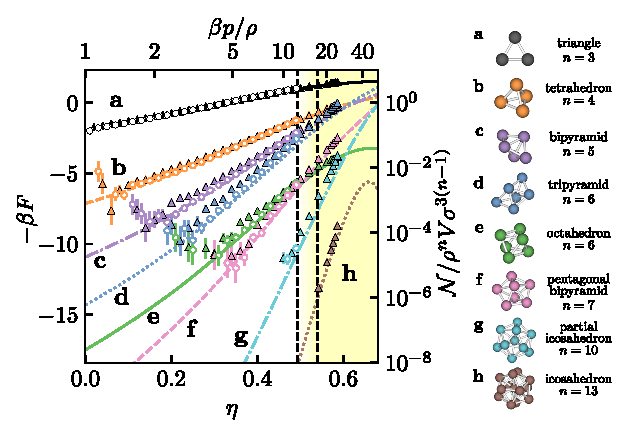
\includegraphics[width=\linewidth,center]{structure-populations}
  \caption[Concentration of local structures in the equilibrium liquid]{
    Static many-body structure in the hard sphere liquid: populations of small local structures in the hard sphere liquid determined from molecular dynamics simulations of 1372 monodisperse (open circles) and 8\% polydisperse (solid triangles) hard spheres against the theoretical prediction of this chapter (lines).
    Variations against volume fraction $\eta$ and compressibility $Z = \beta p/\rho$ shown.
    The hard sphere freezing and melting volume fractions are indicated by vertical dashed lines.
  }
  \label{fig:structure-populations}
\end{SCfigure}

To demonstrate the effectiveness of this approach we have taken structures for $3 \le n \le 13$ which are global minima of clusters in different simple liquids \cite{Wales2004}.
This set includes frustrated structures for $n \ge 7$ which do not correspond to rigid packings with unique energy minima; we will return to the rigid packings afterwards.
We selected these structures because we can identify them in molecular dynamics simulations using the algorithm of Ref.\ \cite{MalinsTCC2013}.
Using this algorithm we can compare the theoretical predictions against molecular dynamics simulations of both mono- and moderately polydisperse hard spheres at all volume fractions accessed by the simulations i.e.\ $\eta \lesssim 0.585$.
For the polydisperse simulations we used data from Ref.\ \cite{RoyallJSM2017} with a 5-component equimolar distribution with $\sim8\%$ polydispersity, to avoid freezing at high densities, and for the monodisperse simulations we used the DynamO software for event-driven molecular dynamics \cite{BannermanJCC2011}.
We determined their free energies using the thermodynamic integration steps outlined above.

\begin{SCfigure}
  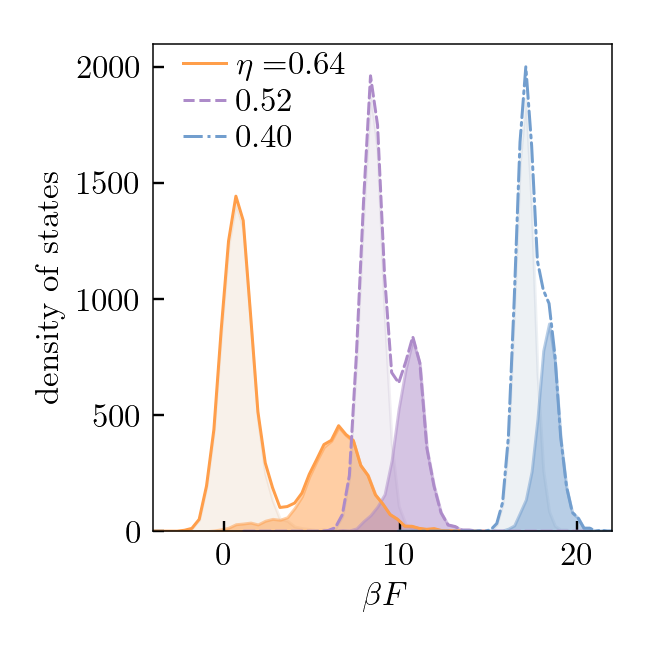
\includegraphics[width=0.9\linewidth,outer]{n12-dos}
  \caption[Free energy distribution of 12 particle structures]{
    Theoretical free energy distribution for the $n=12$ local library of states at several volume fractions.
    The distribution is shifted to lower energies at higher volume fractions, and develops an increasingly bimodal structure.
    Populations are decomposed into those structures containing pentagonal bipyramids without octahedra (light fill) and the remaining structures (dark fill).
  }
  \label{fig:n12-dos}
\end{SCfigure}

In Fig.\ \ref{fig:structure-populations} we find excellent agreement between the theoretical prediction and the observed concentration of local structure seen in the simulations.
Our approach is able to predict populations of local structures well beyond the regime dynamically accessible to simulation, finding nontrivial structural change deep in the glassy regime highlighted by a rescaling with respect to the trivial $\rho^n$ density contribution.
The free energy of considered structures changes approximately linearly across the entire liquid regime, with deviations from linear becoming more apparent in the supercooled regime.

All structures apart from the fourfold symmetric octahedron in Fig.\ \ref{fig:structure-populations} are subunits of the icosahedron, and increase in concentration more rapidly than the octahedron until high density.
For $n=6$ we consider the free energies of two structures: the tripyramid and octahedron.
We find that the tripyramid occurs $\sim20$ times more often than the octahedron, their free energy difference being dominated by the different point group symmetries \cite{MalinsJPCM2009,MengS2010,CatesSM2015}.
We can also estimate vibrational contributions, which allow us to match not only the relative but also the absolute values of free energies obtained from simulation.
In particular, we are able to capture the gradual reduction of the population of octahedral motifs in favour of the tripyramids at high volume fractions.
This is related to the previously observed emergence of fivefold symmetric motifs (such as the full and partial icosahedron) \cite{RoyallPR2015,TarjusJPCM2005,HallettNC2018,DunleavyNC2015}, which is here directly predicted from liquid state theory.

Having tested that the theory is accurate for selected geometries, we now take the exhaustive list of 11980 rigid structures for $n=12$ determined in Ref.\ \cite{Holmes-CerfonSR2016} to obtain a local density of states for a given sized inhomogeneity.
We calculated the free energy of all (first-order) rigid structures using \eqref{eq:local-structure-free-energy} (right panel of Fig.\ \ref{fig:structure-populations}), finding a bimodal distribution with two main peaks separated by a free energy difference that increases with increasing volume fraction.
We find the that lower energy distribution consists of structures rich in fivefold (icosahedral) symmetry in the absence of fourfold (octahedral) symmetry.
This shows that the hard sphere liquid is highly frustrated, and would be interpreted as the reason hard spheres make good glassformers in the geometric frustration picture \cite{KivelsonPA1995,TarjusJPCM2005}.
However, this result is potentially compatible with other thermodynamic scenarios like random first-order transition theory (RFOT) \cite{LubchenkoARPC2007}.

Each of the structures correspond to unique contact topologies, but in thermal systems (i.e. with finite gaps between particles) we expect many of them to be indistinguishable as found in Ref.\ \cite{TrombachPRE2018}.
As such, we have likely overestimated the height of the each peak, and especially the lower energy peak which contains more frustrated structures; we will find evidence of this in the next section.
Nevertheless, because this set of packings is exhaustive they represent a complete local density of states in the liquid, which is of fundamental interest to RFOT \cite{LubchenkoARPC2007}.
The distribution of energy levels is a key quantity, but to really examine the connection with dynamics we also need to know the \emph{connectivity} of the different energy states.
For this we need their reaction paths.

We used thermodynamic integration with Monte-Carlo methods to evaluate the free energies in this section, which cannot be straightforwardly applied along reaction paths.
Along reaction paths the geometries are saddles of the potential $\phi^{(n)}$, so the unstable direction must be excluded from integration.
In the next section we introduce analytical methods for evaluating the free energy to address this problem.

%As a Monte-Carlo method it would be very difficult to extend this method to saddles which is of great interest.
%Before moving on to our approximate analytical integration schemes we describe a method which is essentially exact to within numerical precision, at the cost of greater computational expense.

\section{Free energies along reaction paths}
\label{sec:reaction-paths}

While the thermodynamic integration techniques of the previous section are exact in principle, it is desirable to develop analytic approaches for evaluating the free energy.
Analytic approaches are typically faster which is desirable for dealing with larger $n$, as the number of possible packings appears to grow super-exponentially with particle number \cite{Holmes-CerfonSR2016}.
Moreover, analytic approaches are more readily able to calculate free energies along saddles, which are needed to obtain dynamical information in the vein of energy landscape approaches \cite{Wales2004}.

Evaluating the free energy of hard sphere local structures is challenging, because the singular nature of the pair potential requires a non-perturbative treatment.
This effectively corresponds to having non-trivial integration limits.
However, the smoothly varying parts of the integrands can and will be treated perturbatively.

\subsection{Formalism for structure integrals}
\label{sec:analytic-integrals}

The integrals in \eqref{eq:structural-partition-function-detailed} are generically of the form
\begin{equation}\label{eq:schematic-partition-function}
  \mathcal{I}
  =
  \int_{D'}
  %e^{-\beta U_n(\vec{x})} \, y^{(n)}(\vec{x})
  g^{(n)}(\vec{x}) R(\vec{x})
  \, d^l \vec{x},
\end{equation}
where $l = 3n - 6$ and $R(\vec{x}) = \sqrt{\det{\overline{G_{ij}}(\vec{x})} \det{\vec{I}(\vec{x})}}$ is the rotational metric.
The rotational metric is a complicated function as the internal coordinates are curvilinear in general, however we found it to be slowly varying in all of our numerical tests so we can treat it perturbatively.
Treating the combined effect of the distribution function $g^{(n)}$, including the hard sphere interactions, and integration limits of $\mathcal{D'}$ as a probability distribution $\mathcal{P}$ acting over \emph{all} of space, we can formally write
\begin{subequations}
  \begin{align}
    \mathcal{I}
    &=
    Z \int_{\mathbb{R}^l} p(\vec{x}) R(\vec{x}) \, d^l \vec{x},
    \\
    Z
    &=
    \int_{\mathcal{D}'} g^{(n)}(\vec{x}) \, d^l \vec{x},
    \\
    1
    &=
    \int_{\mathbb{R}^l} p(\vec{x}) \, d^l \vec{x},
  \end{align}
\end{subequations}
where $p(\vec{x}) \sim \mathcal{P}$ and $Z$ is the normalisation of the integral in the absence of the metric.

Taylor expanding the metric about the contact point $\vec{x}^*$, i.e.\
\begin{equation*}
  R(\vec{x})
  =
  R(\vec{x}^*)
  + \nabla R(\vec{x}^*) \cdot \Delta \vec{x}
  + \frac{1}{2} \Delta\vec{x} \cdot \nabla \nabla R(\vec{x}^*) \cdot \Delta\vec{x}
  + \mathcal{O}(\Delta\vec{x}^3),
\end{equation*}
where $\Delta \vec{x} = \vec{x} - \vec{x}^*$ leads to the formula
\begin{equation}\label{eq:rotation-metric-perturbations}
  \frac{\mathcal{I}}{Z}
  =
  R(\vec{x}^*)
  + \nabla R(\vec{x}^*) \cdot
  \left\langle \Delta \vec{x} \right\rangle_\mathcal{P}
  + \frac{1}{2} \nabla \nabla R(\vec{x}^*) :
  \left\langle \Delta\vec{x} \otimes \Delta\vec{x} \right\rangle_\mathcal{P}
  + \mathcal{O}(\langle \Delta\vec{x}^3 \rangle_\mathcal{P}),
\end{equation}
with $\langle \cdot \rangle_\mathcal{P} = \int_{\mathbb{R}^l} (\cdot) p(\vec{x}) \, d^l \vec{x}$ as the average over the distribution $\mathcal{P}$.
With this series expansion in mind, we will concentrate on methods which determine $Z$ and the moments of $\mathcal{P}$ to avoid explicitly considering the nonlinear role of the metric $R(\vec{x})$.
This formalism shifts all the complexity into determining approximation schemes for $p(\vec{x})$.

Formally, the probability distribution is written
\begin{equation}
  p(\vec{x})
  =
  \frac{g^{(n)}(\vec{x}) \mathbb{I}_{\mathcal{D}'}(\vec{x})}{Z}
\end{equation}
with indicator function%
\marginfootnote{This is really the Euler characteristic \eqref{eq:euler-characteristic-definition} of the intersection $\chi[\mathcal{D}' \cap \vec{x}]$.}
\begin{equation*}
  \mathbb{I}_{\mathcal{D}'}(\vec{x})
  =
  \begin{cases}
    1 & \textrm{ if } \vec{x} \in \mathcal{D}' \\
    0 & \textrm{ otherwise}.
  \end{cases}
\end{equation*}
The probability distribution contains singularities from both the hard sphere interactions in $g^{(n)}$ and from the integration limits of $\mathcal{D}'$ through $\mathbb{I}_{\mathcal{D}'}$.
Separated into smooth and singular contributions, we can write
\begin{equation*}
  p(\vec{x})
  =
  \underbrace{
    \frac{y^{(n)}(\vec{x})}{Z}
    \vphantom{\prod_{\substack{i < j \\ (i,j) \notin \mathcal{M}}}}
  }_\textrm{smooth}
  \;
  \underbrace{
    \mathbb{I}_{\mathcal{D}'}(\vec{x})
    \prod_{\substack{i < j \\ (i,j) \notin \mathcal{M}}}
    \Theta \Big( |\vec{r}_i - \vec{r}_j| - \sigma \Big)
  }_\textrm{singular terms},
\end{equation*}
where we did not include the particles in $\mathcal{M}$ in the final product because their effect is already by the definition of structure $\mathbb{I}_{\mathcal{D}'}$, and where we defined the $n$-particle cavity distribution as
\begin{equation*}
  \begin{split}
    y^{(n)}(\vec{x})
    :=
    e^{\beta U_n} g^{(n)}(\vec{x}) = e^{-\beta(\Delta\Omega(\vec{x}) - n\mu^\mathrm{ex})},
  \end{split}
\end{equation*}
using \eqref{eq:distribution-solvation} in the latter step.
The cavity distribution is known to be a continuous function \cite{Hansen2013}, so we can perform a perturbation expansion; we will do this to leading order i.e.\
\begin{equation}\label{eq:cavity-perturbation}
  y^{(n)}(\vec{x})
  =
  y^{(n)}(\vec{x}^*) e^{-\vec{A} \cdot \Delta \vec{x}}
  + \mathcal{O}(\Delta \vec{x}^2)
\end{equation}
where $\vec{A} = \nabla \beta\Omega(\vec{x}^*) \ne 0$.
By contrast, the singular terms require a non-perturbative treatment.

The singular terms can be expressed in terms of one-dimensional indicator functions; specifically, our choice of structure laid out in \ref{sec:structure-definition} is a restriction of to the space $h_{ij} \in [0, \delta]$ for particles in contact at the reference point $\vec{x}^*$, and the full space $[0, \infty]$ for the remaining particle pairs.
We write this as
\begin{subequations}
  \begin{align}
    \mathbb{I}_{\mathcal{D}'}(\vec{x})
    =
    \prod_{k = 1}^m
    %% \Theta \Big( |\vec{r}_i - \vec{r}_j| - \sigma \Big)
    %% \Theta \Big( \delta - (|\vec{r}_i - \vec{r}_j| - \sigma) \Big)
    \Theta ( h_{a_k b_k} )
    \Theta ( \delta - h_{a_k b_k} )
    &=
    \prod_{(i,j) \in \mathcal{M}} \mathbb{I}_{[0, \delta]} (h_{ij})
  %% \end{equation}
    %% \begin{equation}
    \\
    \prod_{\substack{i < j \\ (i,j) \notin \mathcal{M}}}
    \Theta \Big( |\vec{r}_i - \vec{r}_j| - \sigma \Big)
    &=
    \prod_{\substack{i < j \\ (i,j) \notin \mathcal{M}}}
    \mathbb{I}_{[0, \infty]} (h_{ij}).
  \end{align}
\end{subequations}
So together with \eqref{eq:cavity-perturbation}, the probability distribution becomes
\begin{equation}\label{eq:expanded-structure-p}
  p(\vec{x})
  \simeq
  \frac{y^{(n)}(\vec{x}^*) e^{-\vec{A} \cdot \Delta \vec{x}}}{Z}
  \,
  %\prod_{k = 1}^m \mathbb{I}_{[0, \delta]}(h_k)
  \prod_{(i,j) \in \mathcal{M}} \mathbb{I}_{[0, \delta]}(h_{ij})
  \prod_{\substack{i < j \\ (i,j) \notin \mathcal{M}}}
  \mathbb{I}_{[0, \infty]} (h_{ij}).
  %% \prod_{\substack{i < j \\ (i,j) \notin \mathcal{M}}}
  %% \mathbb{I}_{[0, \infty]}(|\vec{r}_i - \vec{r}_j| - \sigma).
  %+ \mathcal{O}(\Delta \vec{x}^2)
\end{equation}
In the special case of minimally constrained geometries i.e.\ $m = l$, then the integration limits are equivalent to a hypercube.
The resulting integral can be evaluated analytically if the additional hard sphere interactions are ignored (Appendix \ref{appendix:bayesian}).

More generally, we employ two approximations (full details in Appendix \ref{appendix:bayesian}):
\begin{enumerate}
\item \emph{Polyhedral approximation}: we approximate the integration domain as a high dimensional polyhedron.
  \todo{say a bit more here}
\item \emph{Expectation propagation}: inspired by the harmonic approximation \eqref{eq:harmonic-approximation}, we approximate $Z p(\vec{x})$ by an unnormalised Gaussian distribution with parameters obtained using this technique from Bayesian inference described in Refs.\ \cite{Minka2001,MinkaUAI2001,Rasmussen2006,Cunningham2011}.
  This method yields an approximate $Z$, and the Gaussian parameters immediately give the first and second moments of $p(\vec{x})$; the perturbative effects of the rotation metric can thus be included through application of \eqref{eq:rotation-metric-perturbations}.
\end{enumerate}
In the next section we apply this approximate technique to the calculation of free energies along reaction paths.

%% However, the singularity of the pair potential complicates the integral.
%% Note that the limits of the integration $D'$ take care of the hard sphere interactions between the particle pairs in $\mathcal{M}$, but not the remaining interactions.
%% In particular, the hard sphere interaction potential has the form
%% \begin{equation}
%%   e^{-\beta U_N(\vec{x})} =
%%   \prod_{i < j}
%%   \Theta \Big( |\vec{r}_i - \vec{r}_j| - \sigma \Big)
%% \end{equation}
%% where $\Theta(\cdot)$ is the Heaviside theta function.
%% This can be thought of as setting complex integration limits, i.e.\ the additional half-space criterion that $|\vec{r}_i - \vec{r}_j| \in [0, \infty]$.

%% We use two methods:
%% \begin{enumerate}
%% \item Simple: minimally constrained geometries, ignoring $\Theta(\cdot)$
%% \item Expectation propagation (EP): $p(\vec{x})$ is approximated by a Gaussian $q(\vec{x})$ by matching the moment-matching of projections in the directions of the singular subspaces.
%%   See Refs.\ \cite{MinkaUAI2001,Minka2001,Rasmussen2006} for general introductions to EP, and Ref.\ \cite{Cunningham2011} for application to integrations.
%%   Reduces to the first method for minimally constrained geometries where no other hard sphere interactions occur, but more general.
%%   %This method was inspired by the \emph{cavity method} of spin-glasses
%% \end{enumerate}
%% \todo{Write this part.}
%% Loosely speaking, this is the hard-particle analogue of the harmonic approximation with the difference here being that the first derivative does not vanish at the minimum.
%% For $n=6$ this expansion works rather well, as all structures have exactly $3n-6$ bonds and this perturbation theory captures the free energy well when compared with the ``exact'' result from thermodynamic integration.

\subsection{Integration along reaction paths}

%We have two methods
%Two methods: assume no hard sphere interactions outside of the bonded particles, or Bayesian inference
%% \marginfootnote{In the current zeitgeist this could be construed as a form of machine learning; techniques for Bayesian inference are often thrown in with machine learning in e.g.\ topical reviews like Ref.\ \cite{MehtaPR2019}.
%%   Personally, I am hesitant to call this machine learning as the techniques more closely resemble the approximation schemes of traditional statistical mechanics (to me at least) than neural networks which have been driving the recent machine learning revolution.}

\begin{SCfigure}
  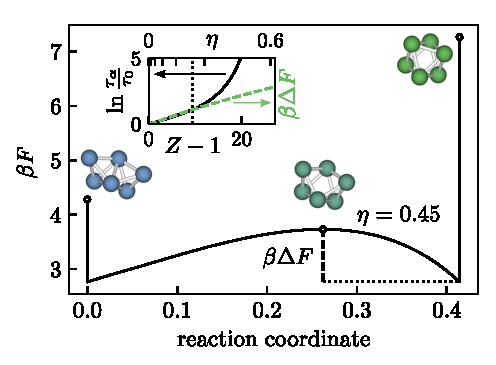
\includegraphics[width=0.9\linewidth,outer]{n6-reaction-path}
  \caption[The simplest nontrivial reaction path in hard spheres: octahedron to tripyramid]{
    Reaction for transition between tripyramid and octahedron $n = 6$ structures.
    Stationary points are indicated by markers: there is a discontinuity in free energy at the end points due to the additional integration over the reaction coordinate, and symmetry in the case of the octahedron.
    Inset: variation of activation barrier with volume fraction $\eta$ and compressibility $Z = \beta p/\rho$ from this theoretical reaction path (dashed line) and measured $\alpha$-relaxation times in bulk molecular dynamics simulations (solid line), where $\eta = 0.45$ is indicated with a vertical dotted line.
  }
  \label{fig:reaction-path-6}
\end{SCfigure}

%We have thus far focused on static thermodynamic properties:
We are now able to make a connection with dynamical properties of the supercooled liquid by calculating the free energy along reaction paths between (geometrically similar) structures.
%This calculation along unstable directions in the free energy landscape requires an analytic approach (described in the SM), and generates paths such as the one in Fig.\ \ref{fig:reaction-path-6}.
We obtain a reaction path by breaking a contact, which creates an unstable direction that can be explored using the technique suggested in the Supplementary Material of Ref.\ \cite{Holmes-CerfonSR2016}.
Along this reaction path we obtain the free energies by integrating over all but the coordinate parameterising the unstable direction $s$.
We therefore obtain from \eqref{eq:structural-partition-function-detailed}
\begin{equation}\label{eq:reaction-path-free-energy}
  \begin{split}
    \beta F
    =&
    %% - \ln \left( \frac{\mathcal{N}}{\sigma^{3(n-1)} \rho^n V},
    %% \\ =&
    - \ln \left(
    \frac{8\pi^2 \sqrt{n^3}}{\nu} \int_{D' \setminus s}
    g^{(n)}(\vec{z}; s) R(\vec{z}; s) \,
    \, d^{l-1} \vec{z}
    \right),
  \end{split}
\end{equation}
where $\vec{z} \in \mathbb{R}^{(3n-7)}$ does not include the reaction coordinate $s$.
Importantly, $\nu$ is the new symmetry number along this reaction path, which is different in general from the symmetry numbers of the terminating minima \cite{Wales2004}.
This integral has the same form as \eqref{eq:schematic-partition-function}, which we evaluate using the methods outlined in the previous section and described in full in Appendix \ref{appendix:bayesian}.
%, i.e.\ by Taylor expansion up to linear terms in the potential and inertia so the integral reduces to a sum of one-dimensional integrals.

In Fig.\ \ref{fig:packings} we see that for $n < 6$ only a single rigid packing of hard spheres exists, but for $n=6$ we see two distinct packings making it the first interesting landscape.
The two structures are connected by a single unstable reaction path, making the entire landscape simple enough to explore.
Comparing this dynamical barrier to the structural relaxation for ($\alpha$-) relaxation timescale $\tau_\alpha$ extracted from simulations relative to a microscopic time $\tau_0$ (inset of Fig.\ \ref{fig:reaction-path-6}), we find this single reaction path barrier agrees with the low density scaling of $\tau_\alpha$ (linear in the compressibility factor $\beta p / \rho$ \cite{BerthierPRE2009}).
However, activated dynamics are not expected in this regime so this agreement may be coincidental.
%Moving to high densities, hard spheres exhibit two-step relaxation when vibrational ($\beta$--) and full ($\alpha$--) relaxations decouple as the system approaches its glass transition \cite{Berthier2011}.
%However, dynamics along the tripyramid--octahedron path continues to increase in an ``Arrhenius'' fashion quite unlike the super-Arrhenius increase exhibited by the $\alpha$--relaxation in the computer simulations (inset of Fig.\ \ref{fig:reaction}).
%It has been shown in molecular systems that $\beta$--relaxation can be Arrhenius in the deeply supercooled regime where $\alpha$-- relaxation is super-Arrhenius \cite{Yu2015}.
%Given that typical particle displacements in the tripyramid--octahedron path are around 0.15$\sigma$ per particle, we observe that this relaxation mechanism may be more characteristic of ($\beta$--) relaxation than full ($\alpha$--) relaxation.

Secondly, we consider the reaction path separating the two variants of the frustrated pentagonal bipyramid with $n=7$ in Fig.\ \ref{fig:reaction-path-7}.
We find that the energy increases monotonically along the path without an activation barrier; this means that these are really thermal fluctuation of the same structure.
%This is not a surprising result, but it opens the way to exploring the for other structures.
This further justifies the use of the frustrated structures in Fig.\ \ref{fig:structure-populations}, even though they do not strictly correspond to unique energy minimum.
On the flip side, it shows that our operational definition of structures needs refining, as we cannot meaningfully distinguish the different energy minima after thermalisation.
This suggests that we have likely overcounted the number of structures in the density of states \ref{fig:n12-dos}.
This calculation relied on expectation propagation \cite{MinkaUAI2001,Minka2001,Rasmussen2006,Cunningham2011} (and Appendix \ref{appendix:bayesian}), which opens the way to assess the connectivity of the energy landscape for local structures in hard spheres.

\begin{SCfigure}
  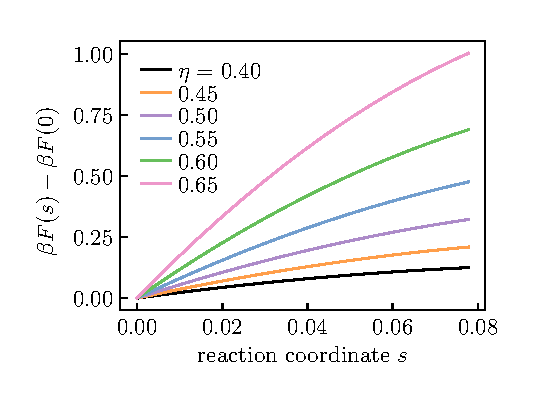
\includegraphics[width=0.9\linewidth,outer]{n7-reaction-path}
  \caption[Reaction path for the two variants of the frustrated pentagonal bipyramid]{
    Reaction for transition between the two $n = 7$ pentagonal bipyramids variant structures, from the variant with a broken spindle (bottom variant in Fig.\ \ref{fig:packings}) to the variant with broken fivefold symmetry (top variant).
    The free energy increases monotonically along this reaction path, so there is no barrier separating these two structures.
  }
  \label{fig:reaction-path-7}
\end{SCfigure}

It is possible to extend our methodology for larger rearrangements, which may be sufficient to access ($\alpha$-) relaxation \emph{at very deep supercooling} for equilibrium systems.
However, the rapid growth in the number of possible states presents a considerable numerical challenge requiring new methods and approximations, so we leave this exciting avenue for future study.

\section{Conclusions}

We have presented a formalism for treating local structure in simple liquids using the framework of many-body correlations.
Using the morphometric approach of the previous chapter, we developed this formalism into an accurate and computationally efficient parameter-free theory for hard spheres relying solely on the equation of state as input.
%This formalism requires knowledge of the energy minima of the potential of mean force to  an operational definition of structures, which could be refined.

We applied the framework to a selection of local structures, therefore predicting nontrivial changes in the energy landscape with supercooling.
This placed previous empirical observations on more solid ground.
In particular, our analysis provides evidence for the existence of two populations of structures with distinct symmetries and free energies which causes the local density of states to become increasingly bimodal at high densities; this observation supports structural interpretations of dynamical arrest.
Examining the reaction pathways we found there was no activation barrier separating two structures with fivefold symmetry, suggesting we have overestimated the number of structures in the lower energy peak.
However, this latter limitation does not challenge the existence of the bimodality caused by an energy separation.

We note that we have treated densities corresponding to a degree of supercooling only accessible using novel swap Monte Carlo techniques \cite{BerthierPRL2016}; however, these simulations introduce large polydispersity, changing the local structure \cite{CoslovichJPCM2018} and thus limiting direct comparison with our calculations for the single-component liquid.

Our framework can be easily adapted to more complex liquids such as systems with soft repulsive interactions and polydisperse mixtures \cite{KodamaJCP2011}.
Calculations may even become easier with softer interactions, as perturbation techniques \eqref{eq:harmonic-approximation} could be used in place of thermodynamic integration, or the bespoke analytic techniques presented in this chapter.
However, extending the approach to softer interactions would require new morphometric coefficients as input to the theory.
This suggests a route for predicting static properties of equilibrium liquids, with direct applications to self-assembly, nucleation and protein structure.

The morphometric approach can extend straightforwardly to hard particles of more complex shapes where the interaction potential is still geometric in nature; in the next chapter we will derive a morphometric theory for arbitrary mixtures of hard convex particles.
The downside of this extension is that this introduces rotational degrees of freedom for each particle, and more complex interactions, so evaluating free energies is likely to become substantially more complicated.

%% \section{New notes.}

%% We wish to describe local structure.
%% Ultimately, we wish to learn about the structure of the energy landscape in hard spheres.
%% To do so we must characterise the main features of the landscape, namely the different geometric packings and assign weights (free energies) to them.
%% This is a worthy goal in its own right, perhaps not that interesting for hard spheres but useful for wider applications (e.g.\ predicting self assembly, guiding chemical synthesis, understanding protein folding kinetics and predicting the native state and design).

%% The path we take is as follows:
%% \begin{enumerate}
%% \item We need some means of weighting points in the energy landscape: we do this using the morphometric approach (cf previous chapter)
%% \item A means of characterising and approximating the entire phase space: energy landscape formalism (next). This has two subgoals:
%%   \begin{enumerate}
%%   \item Divide the landscape into stationary points: minima and saddles.
%%     These stationary points characterise submanifolds of the entire landscape, \emph{basins} in the case of minima and \emph{reaction paths} in the case of saddles.
%%   \item Integrate over connected manifolds with weight function (potential of mean force) to obtain their free energies.
%%   \end{enumerate}
%% \end{enumerate}

%% %Another way of saying this is we need an integrand and boundary conditions.

%% \subsection{Connection with energy landscape descriptions}

%% \begin{itemize}
%%   \item First describe the energy landscape description.
%%   \item Based on low-temperature expansion arguments.
%%   \item Mean-field: Laplace method/saddle-point.
%%   \item Gaussian expansion around this result (called Harmonic approximation in energy landscape/chemistry literature).
%% \end{itemize}

%% %% \begin{SCfigure}[H]
%% %%   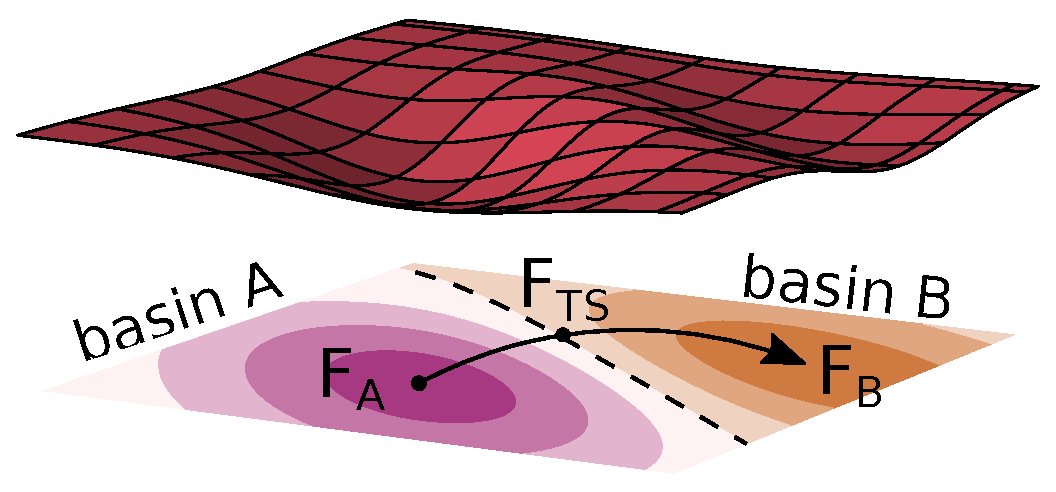
\includegraphics[width=\linewidth,outer]{toy-landscape}
%% %%   \caption[A cartoon energy landscape]{A cartoon energy landscape for a 2-dimensional phase space.
%% %%     The landscape features two local minima: $A$ and $B$.
%% %%     The area surrounding each minima defines its basin: any point from which the minima can be found by moving downhill belongs to the basin.
%% %%     Energy landscape approach: at low temperatures the system is expected to oscillate around potential energy minima, so the dynamics can be understood as rare events causing a change of basin.
%% %%     Thus a decomposition of the phase space in terms of basins should become exact for the dynamics at low temperatures in the supercooled regime of interest.}
%% %% \end{SCfigure}

%% In the case of local arrangements of hard spheres, rigid packings seem to correspond to minima of the potential of mean force.
%% I cannot prove this for the case of morphometric approach, but I cannot find a counter example.
%% Possibly can prove they are minimal volume.

%% \section{Locally favoured structures in hard spheres}

%% \section{Introduction}

%% This study builds on and contributes to work in nonequilibrium statistical physics, particularly relating to glasses and nucleation.
%% Although small-system studies have examined how dynamics are influenced by topographical properties of the energy landscape for simple systems, there has not been a systematic formalism for extending this to the bulk liquid.
%% As such, this study provides additional insight into dynamical arrest i.e.\ the supercooled liquid and glasses.

%% The analytic focus on many-body correlations provides another contribution to the fundamental understanding of simple liquids.
%% This study analyses depletion forces in order to predict the many-body correlation functions in the bulk liquid.
%% Although numerous studies have identified the role of local structure in dynamical arrest little analytical attention has been paid to how to properly formulate structure in a quantitative thermodynamic framework.
%% I address this issue by expressing the solvation free energies in terms of geometrical properties of a small solute, and develop techniques for making quantitative predictions of local structure in the hard sphere liquid.

%% Energy landscape can be divided into two strands: the topographic view of Stillinger which offers a powerful conceptual tool for understanding complex phenomena.
%% At low temperatures we can imagine the system oscillating around low energy minima (inherent states), with occasional large fluctuations driving it through `choke points' causing a change to a different energy minimum.
%% This formalism was turned into a properly quantitative framework by Wales \cite{Wales2004,?}, where stationary point databases are constructed: energy minima connected by saddles.
%% From the connectivity of the landscape one can understand dynamical arrest: if there are lots of competing low lying minima it can be hard for the system to find the global minimum and we expect it to fall out of equilibrium easily when temperature is lowered.
%% By contrast, if the minima steadily lower in energy then they act as a funnel to the global minimum so we expect rapid equilibration.

%% Quantitative predictions are typically only possible for small systems, so it is desirable to extend it to the bulk.
%% One can to do this focusing on a subset of the total degrees of freedom, integrating out the rest in an approximate fashion.
%% The selected degrees of freedom act as a small system with a many-body interaction potential, so can be treated with the aforementioned formalism in a quantitative manner.
%% This was attempted by Tarjus \cite{?} with mixed success.
%% The morphometric approach \cite{KonigPRL2004,RothPRL2006,RobinsonPRL2019} offers a generic framework to treat many-body correlations allowing a first-principles treatment of local structure in the bulk liquid.
%% This framework is accurate for hard spheres where it has been extensively tested \cite{Hansen-Goos?,Roth?,Bob?,RobinsonPRL2019}.

%% Hard particle systems are the fundamental system of interest for simple liquids.
%% The stationary point database approach, firmly rooted in \emph{potential energy}, fails for hard systems as the potential energy is trivial so the thermodynamics is athermal.
%% It has never been extended to hard systems until now.
%% This extension comes with the cost that some of the elegant techniques of soft systems will fail due to the singular nature of hard sphere interactions, so we require new methods to handle the idiosyncrasies of hard systems.
%% Here we propose a practical definition for basins when working with hard systems, and develop techniques for evaluating thermodynamic quantities with this definition.
%% We then retroactively justify the meaningfulness of this basins by comparing with simulation/literature data.

%% \todo{Talk about the past work on hard spheres: penny packing, and sticky spheres.}
%% A number of unique technical challenges brought about by the hard sphere potential, that we will solve.
%% The groundwork for this was laid down by Holmes-Cerfon and coworkers.
%% Note: attempts have been successful at modelling effective interactions close to isostaticity where $z \to 2d$.
%% This is empirically found to be the case asymptotically as one approaches jamming, however it is worth noting that there is no general requirement that $z = 2d$ for rigid packings, and counter examples where $z < 2d$ are known.

%% In section \ref{sec:energy-landscapes} we review the energy landscape formalism for soft potentials, with a view to highlighting where it might fail for hard interactions.
%% We review the liquid state theory/morphological approach used for treating the depletion interactions between hard particles in the bulk liquid in section \ref{?},
%% followed by the equivalent of the partition function for local structure.
%% Our core theoertical results are then presented in section \ref{?}, where we propose a definition of local structure and show techniques for evaluating the partition function nonperturbatively.
%% We then present the results of the topography of the local structural energy landscape in hard spheres in section \ref{?}, our main numerical results.

%% \section{Energy landscape approaches}
%% \label{sec:energy-landscapes}

%% Points to cover:
%% \begin{itemize}
%% \item Give a technical definition of local structure with a goal to showing the problems with hard systems.
%% \item Define structures as manifold: $\mathbb{R}^{dn}$ for $n \ll N$, embedded in $\mathbb{R}^{dN}$
%% \item Failure of perturbation theory due to singularity of
%% \end{itemize}

%% The energy landscape/inherent structure approach is a powerful theoretical framework for understanding complex phenomena.
%% At its core, it is a means of coarse-graining the high dimensional phase space into a more manageable mesostates.
%% Its power comes from the fact that it is essentially exact, though calculations are typically intractable unless the degrees of freedom can be significantly reduced; in practice this is generally only possible in mean field (high spatial dimensions) or for small systems $N = \mathcal{O}(10)$ in physical settings.
%% The approach is however useful conceptually for developing theories based around the topography of the energy landscape \cite{Stillinger}, and makes detailed calculations tractable typically for small systems \cite{Wales2004}.

%% In this section we will review the energy landscape approach, how it applies to soft potentials and the complications that arise for our system of interest: hard spheres.
%% First we talk about coarse-graining into mesostates mentioned above, whether into inherent structures or otherwise.
%% A mesostate is a collection of microstates which are grouped together, typically these are selected for sharing some desirable property to simplify description.
%% For practical reasons this means that microstates should be connected in phase space so they are compact manifolds.
%% In connection with the topographic view we will call these manifolds \emph{basins}.
%% The total partition function is then decomposed as
%% \begin{equation}
%%   Z \equiv \int_{\mathbb{R}^{dN}} e^{-\beta (U_N(\vec{r}^n) + \phi(\vec{r}^n))} \, d\vec{r}^N = \sum_i Z_i
%% \end{equation}
%% where $\phi$ is the external potential of the container in order to keep the particles localised in a region where they interact.
%% Alternatively they could be embedded in a toroidal topology to prevent particle dissociation (as in e.g.\ simulations with periodic boundary conditions).
%% The basin partition function is
%% \begin{equation}
%%   Z_i = \int_{\mathbb{V}_i^{dN}} e^{-\beta U_N(\vec{r}^N)} \, d\vec{r}^N
%% \end{equation}
%% if $\mathbb{V}_i^{dN} \subset \mathbb{R}^{dN}$ is the manifold corresponding to basin $i$.
%% One can define (e.g.\ Wales).
%% Despite a definition which unambiguously demarcates the basins, the high dimensionality of the phase space renders the integrals in \eqref{eq:basin-partition-function} completely intractable without approximation.

%% The equilbrium probability of the system being in basin $i$ at any one time is thus
%% \begin{equation}
%%   p_i = \frac{Z_i}{Z}
%% \end{equation}
%% From the Gibbs-Shannon entropy we find the coarse-graining entropy
%% \begin{equation}
%%   \begin{split}
%%     S_{\textrm{conf}}
%%     &= -\sum_i p_i \ln{p_i} \\
%%     &= -\sum_i \left( \frac{Z_i}{Z} \ln{Z_i} - \frac{Z_i}{Z} \ln{Z} \right) \\
%%     &= \ln{Z} - \sum_i \frac{Z_i}{Z} \ln{Z_i}
%%   \end{split}
%% \end{equation}
%% Noting that the total free energy is $F = -k_B T \ln{Z}$ we thus have
%% \begin{equation}
%%   \beta F = \langle \beta F_i \rangle - S_{\textrm{conf}}
%% \end{equation}
%% where the average basin free energy $F_i = -k_B T \ln{Z_i}$ is
%% \begin{equation}
%%   \langle \beta F_i \rangle = - \frac{1}{Z} \sum_i Z_i \ln{Z_i}
%% \end{equation}

%% Finally, we have to choose how to define the basins.
%% In the energy landscape approach the coarse-graining occurs around local minima of energy where $\nablaU_N = 0$ and Hessian $\frac{1}{2}\nabla\nabla U_N$ is positive definite.
%% Each basin consists of all the points connected by a steepest descent path to a unique energy minimum.
%% This description reduces the high dimensional continuous description down to discrete number of zero-dimensional manifolds.
%% In practice the number of minima scales exponentially in $N$, so this is still an intractably large number of points.
%% One can even obtain dynamical information by considering the saddles, i.e.\ the unstable stationary points.
%% The saddles act as the lowest (in energy) lying points that must be crossed to jump from one basin to another, giving the energy barriers to dynamics.

%% How do we justify this approach?
%% Energy is smooth so asymptotics around stationary points is valid: inherent state (stable stationary points) description
%% For infinite systems we could use Laplace method
%% \begin{equation}
%%   \int_{\mathbb{V}^{dN}_i} e^{-\beta N u_N(\vec{r}^N)} \, d\vec{r}^N
%%   \sim
%%   e^{-\beta \min{U_N(\vec{r}^N)}} \qquad \forall \; N \gg 1
%% \end{equation}
%% where $u_N = U_N / N$.
%% For finite systems we could go beyond this pertubatively by employing a harmonic approximation from the energy-landscape literature
%% \begin{equation}
%%   U_N = U_N(\vec{p}_i) +
%%   \frac{1}{2} \Delta \vec{r} \cdot \left. \nabla \nabla U_N\right|_{\vec{p}_i} \cdot \Delta \vec{r}
%%   + \mathcal{O}(\Delta \vec{r}^3)
%% \end{equation}
%% where \[\vec{p}_i = \argmin_{\vec{r}^n \in \mathbb{V}_i^{dN}}{\left(U_N(\vec{r}^n)\right)}\] is the location of the energy minimum.
%% \begin{equation}
%%   Z_i \sim \exp{-\beta U_N(\vec{p}_i)}
%% \end{equation}
%% There are two layers of approximation: first we model the pdf as a Gaussian, second we approximate the boundary conditions as being infinite.
%% The inclusion of the Hessian term in the expansion around the minimum shows that for soft potentials one can perturbatively build a description around the inherent states.
%% At low temperatures this approach is expected to become exact (for the first layer not the second one).
%% So for athermal systems perturbation theory should break down.

%% \begin{SCfigure}
%%   \missingfigure[figwidth=\linewidth]{}
%%   \caption{Failure of Laplace method for hard interactions.}
%% \end{SCfigure}

%% To make the above discussion concrete we will consider two examples.
%% First, we examine a symmetric quartic potential
%% \begin{equation}
%%   \phi = \epsilon (x^4 - x^2)
%% \end{equation}
%% where $x$ is some state variable and $\epsilon$ is an energy scale.
%% This could represent e.g.\ a ferromagnet below the critical temperature with $x$ representing the spontaneous magnetisation.
%% The free energy in units of $\epsilon$ is then
%% \begin{equation}
%%   F = - T \ln{\left( \int \exp{\left(-\frac{\phi}{T}\right)} \, dx \right)}
%% \end{equation}
%% This potential naturally contains two basins for the two half space $x \in [-\infty, 0]$ and $x \in [0, \infty]$, and because of the symmetry of the potential around $x=0$ the contribution of each of these basins is identical, i.e.\
%% \begin{equation}
%%   Z = 2 \int_0^\infty \exp{\left(-\frac{\phi}{T}\right)} \, dx.
%% \end{equation}
%% Applying the harmonic approximation
%% \begin{equation}
%%   \begin{split}
%%   Z &\simeq
%%   2 \exp{\left( -\frac{\phi(x_0)}{T} \right)}
%%   \int_{-\infty}^\infty \exp{\left(-\frac{\phi''(x_0)}{2T}\right)} \, dx \\
%%   &=
%%   2 \exp{\left( -\frac{\phi(x_0)}{T} \right)}
%%   \sqrt{\frac{2 \pi T}{\phi''(x_0)}}
%%   %+ \mathcal{O}(\phi'''(x_0))
%%   \end{split}
%% \end{equation}
%% where $x_0 = \dfrac{1}{\sqrt{2}}$ is the position of the minimum in the $x > 0$ basin.

%% To summarise this section, we note that the basin definition of structures for soft potentials has the properties that: \cite{Wales?}
%% \begin{itemize}
%% \item Each basin $B_i$ connects to a unique minimal energy state with a unique geometry.
%% \item Divide the phase space into basins which do not overlap $B_i \cap B_j = \emptyset$ for $i \ne j$ and tile the whole of phase space $\cup_i B_i = \mathbb{R}^q$.
%% \item Its free energy is well-defined (at least in some asymptotic limit) so it can be approximated with simple methods.
%%   For soft potentials this is a consequence of the first criterion.
%%   This makes the choice of coarse-graining (thermo)dynamically meaningful: it is long-lived enough that the microstates making up a basin can be not distinguished, and the dynamics reduces to basin crossing events.
%% \end{itemize}
%% A definition satisfying the first two criteria is possible, however due to the singularity in the hard particle interaction potential the region surrounding the (depletion) energy minimum is thermodynamically irrelevant.
%% This can be interpretted:
%% \begin{itemize}
%% \item \emph{Thermodynamically}: the region near contact is entropically suppressed, regions away from contact have many more microstates so are entropically enhanced
%% \item \emph{Dynamically}: as hard spheres approach one another they collide and bounce away so spend infinitesimally small timescales at contact.
%%   Collisions almost universally involve only two particles, collisions of more than two particles occur with zero measure.
%% \end{itemize}
%% Because of this we cannot obtain the free energy by a small parameter expansion around the contact point.
%% We must evaluate the full integral over a finite volume.
%% To make this tractable we will abandon the rigorous definition of structures in terms of basins employed for soft potentials, in favour of a simple one based on intuitive geometrical ideas.
%% We will later explore the limitations/successes of this definition in order to retroactively justify this approach.

%% Note that for all of the geometries we have tested this metric seems to be 2, although we could not prove this is in the general case.
%% We have to actually evaluate the integral.
%% We will explore thermodynamic integration using Monte Carlo, which is essentially exact to numerical precision but slow, and some analytical approximations.

%% \subsection{Worked examples}

%% %% \begin{SCfigure}
%% %%   \missingfigure[figwidth=\linewidth]{}
%% %%   \caption{Number of first shell neighbours in the hard sphere liquid.}
%% %% \end{SCfigure}

%% %% \begin{SCfigure}
%% %%   \missingfigure[figwidth=\linewidth]{}
%% %%   \caption{Number of equilateral triangles in the hard sphere liquid.}
%% %% \end{SCfigure}

%% We will consider two worked examples for simple geometries which are readily visualised and for which the metric $G(\vec{x})$ is known exactly and the partition function integral reduces to a simple form.

%% Our first worked example is at the two-body level: the typical number of neighbours in the first shell.
%% For a dimer the metric term evaluates to $G(\vec{x}) = r^2$, i.e.\ the usual spherical coordinate Jacobian as expected.
%% The average number neighbours less than some distance $r$ is then
%% \begin{equation}
%%   z(r)
%%   = 4\pi \int_0^r g^{(2)}(r) r^2 \, dr
%%   = 4\pi \int_\sigma^r e^{-\beta \phi^{(2)}(r)} r^2 \, dr
%% \end{equation}
%% This is a common measurement where $r$ is taken up to the first minimum of the $g(r)$ then $z$ corresponds to the number in the ``first-shell'' (i.e. the coordination number).

%% Our second worked example considers the average concentration of triangles in the liquid.
%% Here the relevant coordinates are the tuple $\vec{x} = (r,s,t)$ where the three distances are the lengths of the triangle.
%% The metric has previously been determined exactly as $G(\vec{x}) = rst$ in \cite{?}.
%% The number of equilateral triangles with maximum side length $\delta$ is then
%% \begin{equation}
%%   N_\Delta(\delta)
%%   =
%%   8\pi^2 \int_\sigma^\delta\int_\sigma^\delta\int_\sigma^\delta
%%   e^{-\beta\phi^{(3)}(r,s,t)} rst \, dr ds dt.
%% \end{equation}
%% The results show excellent agreement with molecular dynamics simulations across the entire liquid regime, and even into the supercooled regime where simulations are available for a polydisperse system.

%% \section{Results}

%% We take the minimal energy structures as the stable packings determined in Refs.\ \cite{ArkusPRL2009,Holmes-CerfonSR2016}.
%% For each landscape with $n \le 5$ there is only a single stable packing, i.e.\
%% \begin{itemize}
%% \item Dimer $n=2$
%% \item Equilateral triangle $n=3$
%% \item Tetrahedron $n=4$
%% \item (Triangular) bipyramid $n=5$
%% \end{itemize}
%% However for $n = 6$ we first see two competing packings: the tritetrahedron and the octahedron.

%% At $n = 7$ there are 5 stable packings, including two subgraphs of the pentagonal bipyramid each with a broken bond: one has a broken spindle, the other a broken ring.
%% This is a well known property of hard sphere packings, and the cause of geometric frustration: it is generally well-established \cite{?,?,?,Robinson?} that 5-fold symmetric structures are lower in (free) energy for simple systems, however they do not tile space perfectly leading to the suppresion of long-range ordering.
%% For soft systems this frustration can be overcome and all of these `contraints' can be satisfied \cite{Frank,Wales}.
%% However, if we look at the one-dimensioinal reaction paths for n=7 we see that there is not thermal barrier separating these two structures.
%% This shows that they should not be distinguished in the liquid regime, showing the limitation of our definition of structure: they are simply thermal fluctuations of one another.
%% We have overcounted the number of stable structures for $n=7$ by one.
%% For similar reasons we have likely overestimated number of structures in n = 12 landscape, but does not change the fact that they are lower in energy

%% Comparing accuracy of analytical integration methods, we find a systematic error increasing with volume fraction likely due to the perturbation in the potential of mean force.
%% For most of the structures the error scales with a similar magnitude and the same sign (see Fig.\ \ref{?}), suggesting a systematic error.
%% Numerical experiments for $g^{(3)}$ show that the main source of error is the order of the expansion, with second-order significantly improving it and third-order being essentially exact.
%% We cannot distinguish the result with the true metric from the that with the approximate metric: this is not a big source of error, at least not for $n=3$ where we can test it.

%% However for a subset of the structures we find that the error has the opposite sign, due to a different source of error: the neglect of additional hard sphere interactions.
%% \todo{Collapse all the data onto a single figure.
%%   Can we rescale the error by the free energy?
%%   What can we correlate?}
%% Using expectation propagation the sign of the error is restored showing that we are treating these interactions, though the error is generally larger than for the other structures as it is not an exact method.
%% \todo{Can we include the potential expansion to second order?}

%% \begin{SCtable}
%%   \begin{minipage}[b]{\linewidth}
%%     \centering
%%     \begin{tabular}{cccc}
%%       Structure & $\beta F(\eta=0.45)$ & $\beta F(\eta=0.56)$ & $\beta F(\eta=0.64)$ \\
%%       \hline
%%       1 & 0.5 & 0.7 & 0.9 \\
%%       2 & 0.5 & 0.7 & 0.9 \\
%%       3 & 0.5 & 0.7 & 0.9 \\
%%       4 & 0.5 & 0.7 & 0.9 \\
%%       5 & 0.5 & 0.7 & 0.9 \\
%%     \end{tabular}
%%   \end{minipage}
%%   \caption{Free energies of structures for $n=7$ landscape at varying volume fractions.}
%% \end{SCtable}

%% \begin{SCfigure}
%%   \missingfigure[figwidth=\linewidth]{}
%%   \caption{Distribution of energy levels for $n \le 9$.
%%   Include saddles.}
%% \end{SCfigure}

%% \begin{SCfigure}
%%   \missingfigure[figwidth=\linewidth]{}
%%   \caption{Distribution of energy levels for $10 \le n \le 12$.}
%% \end{SCfigure}

%% Next we give the minimal energy structures for $8 \le n \le 12$.

%% \section{Discussion}

%% Here we summarise our many layers of approximations.
%% First, we have to make a \emph{choice} over how to coarse-grain the phase space.
%% This is not strictly an approximation, but it defines what we mean by a `structure' and informs the approximations used to compute the free energies.
%% Then, we make the following approximations:
%% \begin{enumerate}
%% \item Morphological approach for correlations:
%%   \begin{enumerate}
%%   \item Morphometric \emph{ansatz}
%%   \item Virial choice of closure with Carnahan-Starling equation of state
%%   \end{enumerate}
%% \item Expansions of geometrical measures:
%%   \begin{enumerate}
%%   \item Second-order expansion of geometric measure (i.e.\ moment of inertia)
%%   \item Contact measure for bond-distance space (i.e.\ zeroth-order term): this seems to be more or less exact for $n=3$
%%   \end{enumerate}
%% \item First-order expansion of potential around contact (can we get second?)
%% \item Polyhedral approximation of boundary conditions (additional hard sphere bonds).
%% \item Bayesian inference to perform integral
%% \end{enumerate}
%% \todo{Mention how we nudge the coordinates with a small perturbation from the contact point to prevent problems with e.g.\ four-particle intersections (and higher)}

%% We found that two 5-fold symmetric structures at $n=7$, both pentagonal bipyramids with broken symmetries, are not separated by a thermodynamic barrier.
%% This means they should be considered as thermal fluctuations of one another, and not be distinguished.
%% This explains why 5-fold symmetric structures like the icosahedron are thermally stable in the hard sphere liquid.
%% Note that at jamming the symmetry of these structures must be broken.

\ifdefined\includebibliography
  \newgeometry{margin=1in}
  \printbibliography
\fi

\end{document}
